% Graphical abstract concept 1: the barrier as idle time.
% Two worker timelines with the SAME multiset of simulation durations: the
% synchronous panel waits for the slowest simulation of every generation, the
% asynchronous panel packs every lane. The completed-simulation counts are
% computed in the picture itself, so they are consistent with the drawing.
\documentclass[tikz,border=4pt]{standalone}
\usepackage{newtxtext,newtxmath}
\usetikzlibrary{patterns,decorations.pathreplacing,calc,arrows.meta}
\definecolor{async}{HTML}{0072B2}
\definecolor{sync}{HTML}{D55E00}

\newcounter{syncdone}
\newcounter{asyncdone}

\begin{document}
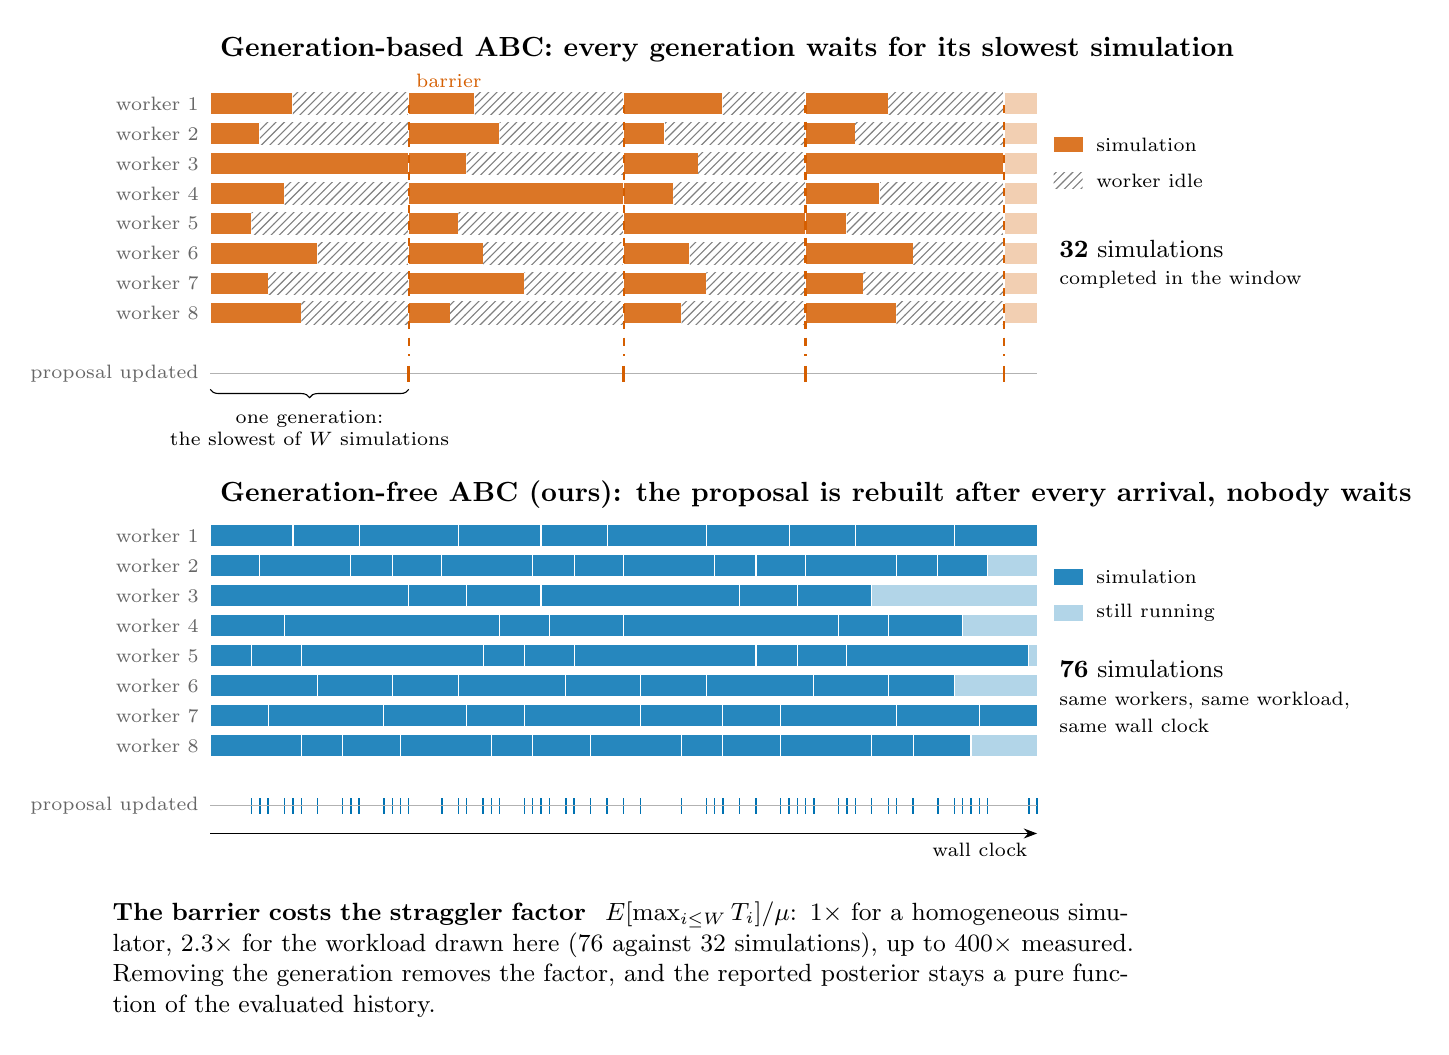
\begin{tikzpicture}[x=1.05cm,y=1cm,font=\small,>=Stealth]
\pgfmathsetmacro{\T}{10}          % wall-clock window, time units
\pgfmathsetmacro{\laneh}{0.28}
\pgfmathsetmacro{\lanegap}{0.10}
% 8 workers x 3 generations of simulation durations (the workload); generation 4+
% recycles column 1, 2, ... so both panels draw from the same multiset.
\def\durations{{{1.0,0.8,1.2},{0.6,1.1,0.5},{2.4,0.7,0.9},{0.9,2.6,0.6},{0.5,0.6,2.2},{1.3,0.9,0.8},{0.7,1.4,1.0},{1.1,0.5,0.7}}}
% barrier times = cumulative slowest simulation per generation: 2.4, 2.6, 2.2, 2.4
\def\barriers{{0,2.4,5.0,7.2,9.6,12.0}}

%% ---------------------------------------------------------------- synchronous
\begin{scope}
\node[anchor=south west,font=\bfseries] at (0,0.55) {Generation-based ABC: every generation waits for its slowest simulation};
\foreach \w in {1,...,8} {
  \pgfmathsetmacro{\yb}{-(\w-1)*(\laneh+\lanegap)}
  \pgfmathsetmacro{\yt}{\yb+\laneh}
  \node[anchor=east,font=\scriptsize,text=black!60,inner sep=1pt] at (-0.1,{(\yb+\yt)/2}) {worker \w};
  \foreach \g in {1,...,5} {
    \pgfmathsetmacro{\Bprev}{\barriers[\g-1]}
    \pgfmathsetmacro{\Bnext}{\barriers[\g]}
    \pgfmathsetmacro{\col}{int(mod(\g-1,3))}
    \pgfmathsetmacro{\d}{\durations[\w-1][\col]}
    \pgfmathsetmacro{\te}{min(\Bprev+\d,\T)}
    \pgfmathsetmacro{\ti}{min(\Bnext,\T)}
    \ifdim \Bprev pt<\T pt
      \ifdim \te pt<\T pt
        \fill[sync!85,draw=white,line width=0.4pt] (\Bprev,\yb) rectangle (\te,\yt);
        \stepcounter{syncdone}
      \else
        \fill[sync!30,draw=white,line width=0.4pt] (\Bprev,\yb) rectangle (\T,\yt);
      \fi
      \ifdim \te pt<\ti pt
        \fill[pattern=north east lines,pattern color=black!50] (\te,\yb) rectangle (\ti,\yt);
      \fi
    \fi
  }
}
\pgfmathsetmacro{\ybot}{-8*(\laneh+\lanegap)+\lanegap}
\foreach \B in {2.4,5.0,7.2,9.6} {
  \draw[sync,dashed,line width=0.8pt] (\B,0.12) -- (\B,\ybot-0.12);
}
\node[anchor=south west,font=\scriptsize,text=sync,inner sep=1pt] at (2.45,0.30) {barrier};
% proposal-update row
\node[anchor=east,font=\scriptsize,text=black!60,inner sep=1pt] at (-0.1,\ybot-0.35) {proposal updated};
\draw[black!30] (0,\ybot-0.35) -- (\T,\ybot-0.35);
\foreach \B in {2.4,5.0,7.2,9.6} { \draw[sync,line width=1pt] (\B,\ybot-0.25) -- (\B,\ybot-0.45); }
% brace for one generation
\draw[decorate,decoration={brace,mirror,amplitude=3pt}] (0,\ybot-0.55) -- (2.4,\ybot-0.55)
  node[midway,below=4pt,font=\scriptsize,align=center] {one generation:\\the slowest of $W$ simulations};
% idle callout
\fill[sync!85] (\T+0.2,{-1.0*(\laneh+\lanegap)-0.1}) rectangle +(0.35,0.2);
\node[anchor=west,font=\scriptsize] at (\T+0.6,{-1.0*(\laneh+\lanegap)}) {simulation};
\fill[pattern=north east lines,pattern color=black!50] (\T+0.2,{-2.2*(\laneh+\lanegap)-0.1}) rectangle +(0.35,0.2);
\node[anchor=west,font=\scriptsize] at (\T+0.6,{-2.2*(\laneh+\lanegap)}) {worker idle};
\node[anchor=west,align=left] at (\T+0.15,{-5.0*(\laneh+\lanegap)}) {\textbf{\arabic{syncdone}} simulations\\[-1pt]{\scriptsize completed in the window}};
\end{scope}

%% --------------------------------------------------------------- asynchronous
\pgfmathsetmacro{\yshift}{-8*(\laneh+\lanegap)-2.45}
\begin{scope}[shift={(0,\yshift)}]
\node[anchor=south west,font=\bfseries] at (0,0.36) {Generation-free ABC (ours): the proposal is rebuilt after every arrival, nobody waits};
\foreach \w in {1,...,8} {
  \pgfmathsetmacro{\yb}{-(\w-1)*(\laneh+\lanegap)}
  \pgfmathsetmacro{\yt}{\yb+\laneh}
  \node[anchor=east,font=\scriptsize,text=black!60,inner sep=1pt] at (-0.1,{(\yb+\yt)/2}) {worker \w};
  \xdef\tcur{0}
  \foreach \j in {0,...,30} {
    \pgfmathsetmacro{\col}{int(mod(\j,3))}
    \pgfmathsetmacro{\d}{\durations[\w-1][\col]}
    \pgfmathsetmacro{\ts}{\tcur}
    \pgfmathsetmacro{\te}{\ts+\d}
    \ifdim \ts pt<\T pt
      \ifdim \te pt>\T pt
        \fill[async!30,draw=white,line width=0.4pt] (\ts,\yb) rectangle (\T,\yt);
      \else
        \fill[async!85,draw=white,line width=0.4pt] (\ts,\yb) rectangle (\te,\yt);
        \draw[async,line width=0.5pt] (\te,{-8*(\laneh+\lanegap)+\lanegap-0.25}) -- (\te,{-8*(\laneh+\lanegap)+\lanegap-0.45});
        \stepcounter{asyncdone}
      \fi
    \fi
    \xdef\tcur{\te}
  }
}
\pgfmathsetmacro{\ybot}{-8*(\laneh+\lanegap)+\lanegap}
\node[anchor=east,font=\scriptsize,text=black!60,inner sep=1pt] at (-0.1,\ybot-0.35) {proposal updated};
\draw[black!30] (0,\ybot-0.35) -- (\T,\ybot-0.35);
\fill[async!85] (\T+0.2,{-1.0*(\laneh+\lanegap)-0.1}) rectangle +(0.35,0.2);
\node[anchor=west,font=\scriptsize] at (\T+0.6,{-1.0*(\laneh+\lanegap)}) {simulation};
\fill[async!30] (\T+0.2,{-2.2*(\laneh+\lanegap)-0.1}) rectangle +(0.35,0.2);
\node[anchor=west,font=\scriptsize] at (\T+0.6,{-2.2*(\laneh+\lanegap)}) {still running};
\node[anchor=west,align=left] at (\T+0.15,{-5.0*(\laneh+\lanegap)}) {\textbf{\arabic{asyncdone}} simulations\\[-1pt]{\scriptsize same workers, same workload,}\\[-1pt]{\scriptsize same wall clock}};
% time axis
\draw[->] (0,\ybot-0.7) -- (\T,\ybot-0.7) node[below left,font=\scriptsize] {wall clock};
\end{scope}

%% ------------------------------------------------------------------- bottom line
\pgfmathsetmacro{\ybl}{\yshift-8*(\laneh+\lanegap)-1.35}
\node[anchor=north west,align=left,text width=13.2cm] at (-1.3,\ybl) {%
  \textbf{The barrier costs the straggler factor} $\;\mathbb{E}[\max_{i\le W}T_i]/\mu$: $1\times$ for a homogeneous simulator,
  $2.3\times$ for the workload drawn here ($\arabic{asyncdone}$ against $\arabic{syncdone}$ simulations), up to $400\times$ measured. Removing the generation removes the factor,
  and the reported posterior stays a pure function of the evaluated history.};
\end{tikzpicture}
\end{document}
